% !TEX root = ../main.tex
% 本文件由 build-tex.sh 从 17-DSP指南-第17章中译.md 生成，改内容请改 md 后重新生成

\chapter{自定义滤波器}\label{ch-17}

大多数滤波器的频率响应属于四种标准类型之一：低通、高通、带通或带阻。本章介绍一种通用方法，用来设计具有任意频率响应的数字滤波器，按你具体应用的需要量身定做。DSP
在这方面表现出色，能解决远远超出模拟电子学能力的问题。本章讨论自定义滤波器的两个重要用途：反卷积(deconvolution)，即恢复经历过不想要的卷积的信号；以及最优滤波(optimal
filtering)，即分离频谱相互重叠的信号的问题。这是 DSP 最精彩的地方。

\section{任意频率响应}

上一章推导加窗 sinc 滤波器(windowed-sinc
filter)的方法，也可以用来设计几乎任何频率响应的滤波器。唯一的区别在于怎样把期望的响应从频域搬到时域。在加窗
sinc
滤波器中，频率响应和滤波器核都用公式表示，两者之间的转换靠计算傅里叶变换的数学来完成。而在这里介绍的方法中，两个信号都用数字数组表示，用一个计算机程序（FFT）由其中一个求出另一个。

图 17-1 是一个例子，说明这个方法怎样运作。我们想让滤波器产生的频率响应如
(a)
所示。说得客气点，它非常不规则，用模拟电子学几乎不可能做到。这个理想频率响应由一组挑选出来的数字定义，而不是某个数学公式。本例中，在采样率的
0 到 0.5 之间分布着 513
个采样。可以用更多的点来更好地表示期望的频率响应，也可能需要用更少的点来缩短滤波器设计时的计算时间。不过，这些顾虑通常都不大，513
对大多数应用来说是个合适的长度。

除了 (a)
所示的期望幅度数组，还必须有一个同样长度的相位数组与之对应。本例中，期望频率响应的相位全为零（图
17-1
没有画出这个数组）。和幅度数组一样，相位数组也可以装入任何你想让滤波器产生的曲线。不过要记住，相位数组的第一个和最后一个采样（即第
0 和第 512 个）的值必须为零（或者 2π
的整数倍，这是一回事）。频率响应也可以用直角坐标形式指定，即给出实部和虚部数组的各项，而不用幅度和相位。

下一步是做逆
DFT，把滤波器搬到时域。最快的办法是把频域转换成直角坐标形式，然后用逆
FFT。得到一个从 0 到 1023 的 1024 点信号，如 (b)
所示。这就是与我们想要的频率响应相对应的冲激响应；不过，它并不适合直接用作滤波器核（稍后详谈）。和上一章一样，它需要经过平移、截断和加窗。本例中，我们设计
\(M = 40\) 的滤波器核，即从第 0 到第 40 个采样共 41 个点。表 17-1
给出了把 (b) 中的信号变成 (c) 所示滤波器核的程序。和加窗 sinc
滤波器一样，滤波器核两端附近的点非常小，画出来看起来就是零。千万别误以为可以把它们删掉！

\textbf{表 17-1}（注释已译成中文）

\begin{Shaded}
\begin{Highlighting}[]
\NormalTok{100 \textquotesingle{}CUSTOM FILTER DESIGN（自定义滤波器设计）}
\NormalTok{110 \textquotesingle{}本程序把一个 1024 点的混叠冲激响应转换成 M+1 点的}
\NormalTok{120 \textquotesingle{}滤波器核（例如把图 17{-}1b 转换成图 17{-}1c）}
\NormalTok{130 \textquotesingle{}}
\NormalTok{140 DIM REX[1023]                      \textquotesingle{}REX[ ] 存放要转换的信号}
\NormalTok{150 DIM T[1023]                        \textquotesingle{}T[ ] 是临时存储缓冲区}
\NormalTok{160 \textquotesingle{}}
\NormalTok{170 PI = 3.14159265}
\NormalTok{180 M\% = 40                            \textquotesingle{}设定滤波器核长度（共 41 个点）}
\NormalTok{190 \textquotesingle{}}
\NormalTok{200 GOSUB XXXX                         \textquotesingle{}虚构的子程序，把冲激响应载入 REX[ ]}
\NormalTok{210 \textquotesingle{}}
\NormalTok{220 FOR I\% = 0 TO 1023                 \textquotesingle{}把信号向右平移（循环移位）M/2 点}
\NormalTok{230 INDEX\% = I\% + M\%/2}
\NormalTok{240 IF INDEX\% \textgreater{} 1023 THEN INDEX\% = INDEX\%{-}1024}
\NormalTok{250 T[INDEX\%] = REX[I\%]}
\NormalTok{260 NEXT I\%}
\NormalTok{270 \textquotesingle{}}
\NormalTok{280 FOR I\% = 0 TO 1023}
\NormalTok{290 REX[I\%] = T[I\%]}
\NormalTok{300 NEXT I\%}
\NormalTok{310 \textquotesingle{}                                  \textquotesingle{}截断信号并加窗}
\NormalTok{320 FOR I\% = 0 TO 1023}
\NormalTok{330 IF I\% \textless{}= M\% THEN REX[I\%] = REX[I\%] * (0.54 {-} 0.46 * COS(2*PI*I\%/M\%))}
\NormalTok{340 IF I\% \textgreater{} M\% THEN REX[I\%] = 0}
\NormalTok{350 NEXT I\%}
\NormalTok{360 \textquotesingle{}                                  \textquotesingle{}滤波器核现在位于 REX[0] 到 REX[40]}
\NormalTok{370 END}
\end{Highlighting}
\end{Shaded}

\textbf{C 实现}（完整可编译版本见
\texttt{c/table17-1\_custom\_filter.c}。原书第 200
行用虚构的子程序载入信号，C 版本把前后两步也补上了：按图 17-1a
的形状定义期望频率响应，逆 DFT 得到混叠冲激响应，执行表
17-1，再求实际频率响应与期望值比较）：

\begin{Shaded}
\begin{Highlighting}[]
\DataTypeTok{static} \DataTypeTok{void}\NormalTok{ custom\_filter\_kernel}\OperatorTok{(}\DataTypeTok{double} \OperatorTok{*}\NormalTok{rex}\OperatorTok{,} \DataTypeTok{int}\NormalTok{ m}\OperatorTok{)}
\OperatorTok{\{}
    \DataTypeTok{double}\NormalTok{ t}\OperatorTok{[}\NormalTok{N}\OperatorTok{];}                            \CommentTok{/* 150 DIM T[1023]：临时缓冲区 */}

    \ControlFlowTok{for} \OperatorTok{(}\DataTypeTok{int}\NormalTok{ i }\OperatorTok{=} \DecValTok{0}\OperatorTok{;}\NormalTok{ i }\OperatorTok{\textless{}}\NormalTok{ N}\OperatorTok{;}\NormalTok{ i}\OperatorTok{++)} \OperatorTok{\{}           \CommentTok{/* 220～260：把信号循环右移 M/2 点 */}
        \DataTypeTok{int}\NormalTok{ index }\OperatorTok{=}\NormalTok{ i }\OperatorTok{+}\NormalTok{ m }\OperatorTok{/} \DecValTok{2}\OperatorTok{;}              \CommentTok{/* 230 */}
        \ControlFlowTok{if} \OperatorTok{(}\NormalTok{index }\OperatorTok{\textgreater{}}\NormalTok{ N }\OperatorTok{{-}} \DecValTok{1}\OperatorTok{)}\NormalTok{ index }\OperatorTok{{-}=}\NormalTok{ N}\OperatorTok{;}      \CommentTok{/* 240：超出末尾的绕回开头 */}
\NormalTok{        t}\OperatorTok{[}\NormalTok{index}\OperatorTok{]} \OperatorTok{=}\NormalTok{ rex}\OperatorTok{[}\NormalTok{i}\OperatorTok{];}                  \CommentTok{/* 250 */}
    \OperatorTok{\}}
    \ControlFlowTok{for} \OperatorTok{(}\DataTypeTok{int}\NormalTok{ i }\OperatorTok{=} \DecValTok{0}\OperatorTok{;}\NormalTok{ i }\OperatorTok{\textless{}}\NormalTok{ N}\OperatorTok{;}\NormalTok{ i}\OperatorTok{++)}             \CommentTok{/* 280～300：拷回 REX[ ] */}
\NormalTok{        rex}\OperatorTok{[}\NormalTok{i}\OperatorTok{]} \OperatorTok{=}\NormalTok{ t}\OperatorTok{[}\NormalTok{i}\OperatorTok{];}

    \ControlFlowTok{for} \OperatorTok{(}\DataTypeTok{int}\NormalTok{ i }\OperatorTok{=} \DecValTok{0}\OperatorTok{;}\NormalTok{ i }\OperatorTok{\textless{}}\NormalTok{ N}\OperatorTok{;}\NormalTok{ i}\OperatorTok{++)} \OperatorTok{\{}           \CommentTok{/* 320～350：截断并加窗 */}
        \ControlFlowTok{if} \OperatorTok{(}\NormalTok{i }\OperatorTok{\textless{}=}\NormalTok{ m}\OperatorTok{)}\NormalTok{ rex}\OperatorTok{[}\NormalTok{i}\OperatorTok{]} \OperatorTok{*=} \FloatTok{0.54} \OperatorTok{{-}} \FloatTok{0.46} \OperatorTok{*}\NormalTok{ cos}\OperatorTok{(}\FloatTok{2.0} \OperatorTok{*}\NormalTok{ PI }\OperatorTok{*}\NormalTok{ i }\OperatorTok{/}\NormalTok{ m}\OperatorTok{);}  \CommentTok{/* 330：汉明窗 */}
        \ControlFlowTok{else}\NormalTok{        rex}\OperatorTok{[}\NormalTok{i}\OperatorTok{]} \OperatorTok{=} \FloatTok{0.0}\OperatorTok{;}           \CommentTok{/* 340：M 之后的点全部置零 */}
    \OperatorTok{\}}
\OperatorTok{\}}                                           \CommentTok{/* 360：滤波器核现在位于 REX[0]～REX[M] */}
\end{Highlighting}
\end{Shaded}

运行结果（实际频率响应与期望频率响应在 513 个设计点上的偏差）：

{\def\LTcaptype{none} % do not increment counter
\begin{longtable}[]{@{}lll@{}}
\toprule\noalign{}
M & 偏差的均方根 & 最大偏差 \\
\midrule\noalign{}
\endhead
\bottomrule\noalign{}
\endlastfoot
10 & 0.399 & 1.33 \\
30 & 0.248 & 0.93 \\
40 & 0.218 & 0.87 \\
100 & 0.125 & 0.76 \\
300 & 0.068 & 0.64 \\
1000 & 0.030 & 0.36 \\
\end{longtable}
}

滤波器核越长，实际响应越贴近期望响应，和图 17-2
的趋势一致；剩下的最大偏差集中在期望响应的陡峭跳变处（比如 0.195 处从
2.5 跌到 1、0.27～0.29
的窄阻带）。程序最后还验证了本节末尾的论点：直接拿 1024
点混叠冲激响应当滤波器核，在 513 个设计点上与期望值的偏差只有
1.8e-13，但在相邻设计点正中间，偏差最大达到 1.49；按表 17-1 加窗后（M =
1000），设计点之间的最大偏差降到 0.098。

\begin{figure}[htbp]
\centering
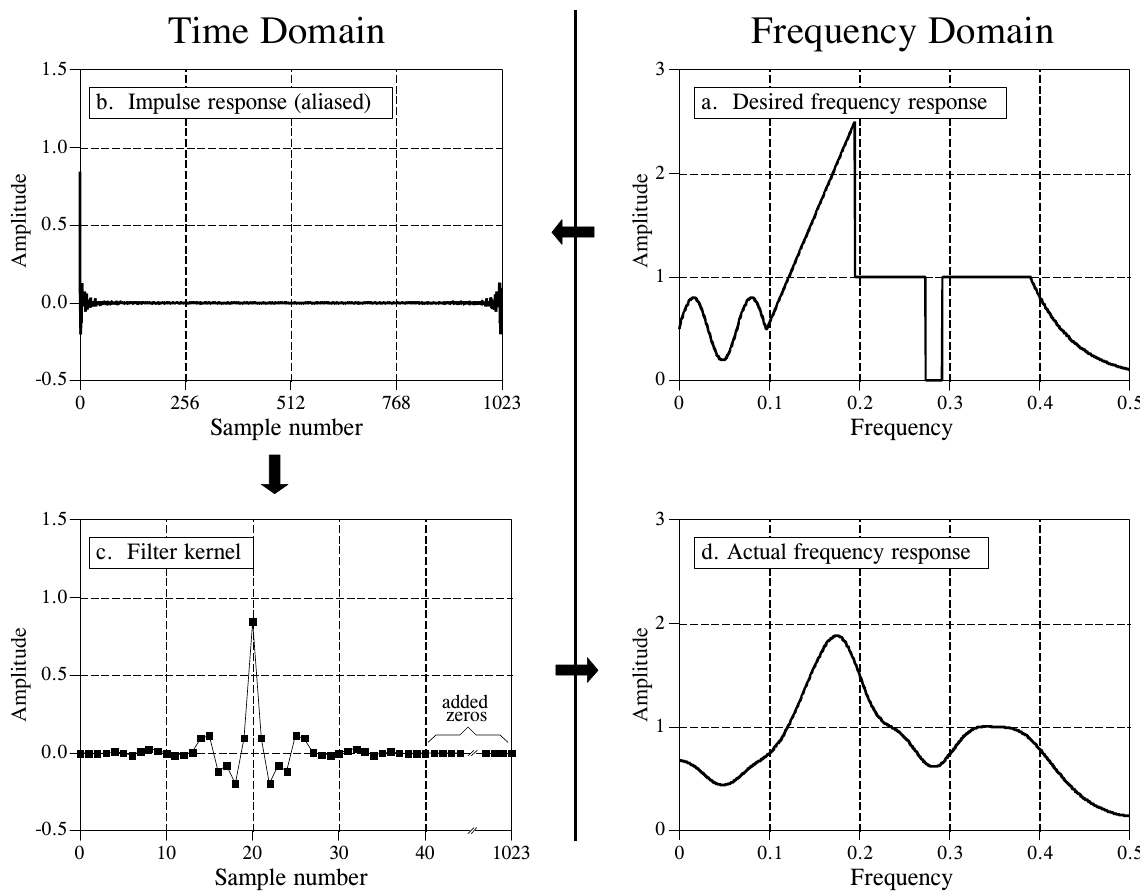
\includegraphics[width=0.950\linewidth,height=0.8\textheight,keepaspectratio]{assets/ch17/fig17-01.png}
\caption*{\textbf{图 17-1　FIR 滤波器设计示例。} (a) 是期望的频率响应，有 513
个采样，分布在采样率的 0 到 0.5 之间。做逆 DFT 得到 (b)，一个由 1024
个采样组成的混叠冲激响应。为了得到滤波器核 (c)，把混叠冲激响应截断为 M+1
个采样、向右平移 M/2 个采样，再乘以汉明窗或布莱克曼窗。本例中 M 为
40。表 17-1 的程序展示了具体做法。检验滤波器核的方法是补零后做
DFT，得到滤波器的实际频率响应 (d)。 （Time Domain = 时域，Frequency
Domain = 频域；a. Desired frequency response = 期望频率响应；b. Impulse
response (aliased) = 冲激响应（混叠的）；c.~Filter kernel =
滤波器核；d.~Actual frequency response = 实际频率响应；added zeros =
补上的零。Amplitude = 幅度，Sample number = 采样序号，Frequency =
频率。图注说''截断\ldots\ldots 再平移''，表 17-1
程序的实际顺序是先平移、后截断。）}
\end{figure}

最后一步是检验滤波器核。做法是做 DFT（用 FFT）求出实际频率响应，如 (d)
所示。为了在频域得到更好的分辨率，在做 FFT
之前给滤波器核补零。例如，总共用 1024 个采样（滤波器核 41 个，加上 983
个零），就能在 0 到 0.5 之间得到 513 个采样。

如图 17-2
所示，滤波器核的长度决定了实际频率响应与期望频率响应吻合得多好。FIR
数字滤波器的出色性能在这里一目了然：只要滤波器核足够长，几乎任何频率响应都能得到。

\begin{figure}[htbp]
\centering
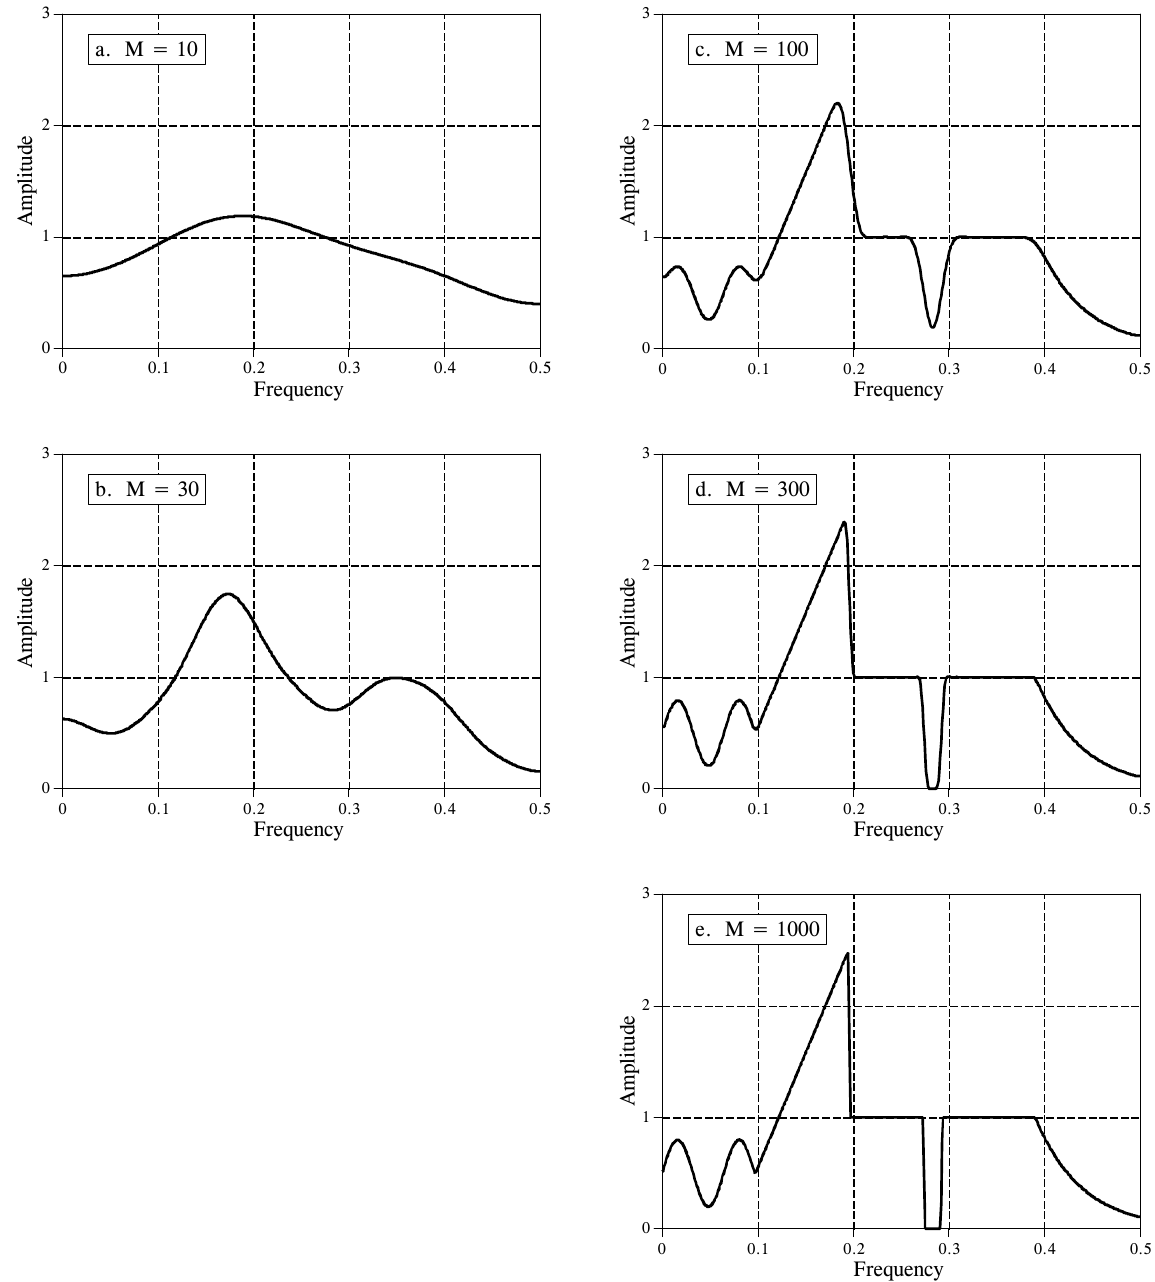
\includegraphics[width=0.963\linewidth,height=0.8\textheight,keepaspectratio]{assets/ch17/fig17-02.png}
\caption*{\textbf{图 17-2　频率响应与滤波器核长度的关系。}
这几张图展示了用不同长度的滤波器核得到的频率响应。每个滤波器核的点数等于
M+1，从 0 到
M。滤波器核用的点越多，得到的频率响应就越接近期望的频率响应。本例的期望频率响应见图
17-1a。 （a～e 依次为 M = 10、30、100、300、1000。Amplitude =
幅度，Frequency =
频率。原书图注排在左下空白处，裁图时已去掉，译文见上。）}
\end{figure}

设计方法就是这些；不过，有一个微妙的理论问题需要澄清。为什么不能直接把图
17-1b 所示的冲激响应用作滤波器核？毕竟，如果 (a) 是 (b)
的傅里叶变换，那么把输入信号与 (b)
卷积，不就能得到我们想要的那个确切的频率响应吗？答案是否定的，原因如下。

设计自定义滤波器时，期望的频率响应由一个数组里的值来定义。现在想一想：在这些指定点之间，频率响应是什么样的？为简单起见，可以设想两种情况，一种''好''，一种''坏''。在''好''的情况下，频率响应在定义的采样之间是一条平滑的曲线。在''坏''的情况下，采样之间有剧烈的起伏。不巧的是，(b)
中的冲激响应对应的恰恰是''坏''的频率响应。这一点可以这样看出：给它补上大量的零，然后做
DFT。用这种方法得到的频率响应，会在原先定义的采样之间表现出不规则的行为，看上去一塌糊涂。

要理解这一点，设想我们在 0 到 0.5
之间无穷多个点上定义频率响应，强迫它就是我们想要的样子。也就是说，我们构造了一条连续曲线。然后用逆
DTFT
求冲激响应，它的长度会是无穷的。换句话说，``好''的频率响应对应着一个计算机无法表示的东西：一个无限长的冲激响应。当我们用
N/2+1 个采样表示频谱时，时域只提供了 N
个点，没法正确容纳这个信号。结果就是，无限长的冲激响应卷绕（混叠）进这 N
个点里。一旦发生这种混叠，频率响应就从''好''变成了''坏''。幸运的是，给这
N 点冲激响应加窗可以大大减轻这种混叠，使频域采样之间成为平滑的曲线。

设计一个产生给定频率响应的数字滤波器相当简单。难的是找出该用什么样的频率响应。我们来看看
DSP 中设计自定义滤波器的一些策略。

\section{反卷积}

不想要的卷积是传输模拟信息时固有的问题。例如，下面这些都可以建模为卷积：手抖的相机拍出的图像模糊、长途电话里的回声、模拟传感器和电子器件的有限带宽，等等。反卷积是对信号做滤波、以补偿不想要的卷积的过程。反卷积的目标是重建卷积发生之前的信号。这通常要求已知卷积的特性（即冲激响应或频率响应）。这一点使它区别于盲反卷积(blind
deconvolution)，后者不知道这个寄生卷积的特性。盲反卷积是困难得多的问题，没有通用的解法，方法必须针对具体应用量身定制。

反卷积在时域几乎无法理解，但在频域却相当直观。构成原信号的每个正弦波，在经过不想要的卷积时，幅度和/或相位都可能改变。要提取原信号，反卷积滤波器必须撤销这些幅度和相位的变化。例如，如果卷积把某个正弦波的幅度变为
0.5 倍、相位移动 30 度，那么反卷积滤波器就必须把这个正弦波放大 2.0
倍、相位改变 −30 度。

我们用来说明反卷积的例子是一个伽马射线探测器(gamma ray detector)。如图
17-3 所示，这种装置由两部分组成：闪烁体(scintillator)和光探测器(light
detector)。闪烁体是一种特殊的透明材料，比如碘化钠或锗酸铋。这些化合物把每个伽马射线的能量转换成一小阵可见光。这些光再由光探测器（比如光电二极管或光电倍增管）转换成电信号。探测器产生的每个脉冲都像一个单边指数函数，只是拐角处略圆一些。这个形状由所用闪烁体的特性决定。伽马射线把能量沉积到闪烁体中时，附近的原子被激发到更高的能级。这些原子随机地退激发，每个产生一个可见光光子。最终的结果是一个光脉冲，它的幅度在几百纳秒内衰减（对碘化钠而言）。由于每个伽马射线的到达都是一个冲激，探测器输出的脉冲（即那个单边指数函数）就是这个系统的冲激响应。

\begin{figure}[htbp]
\centering
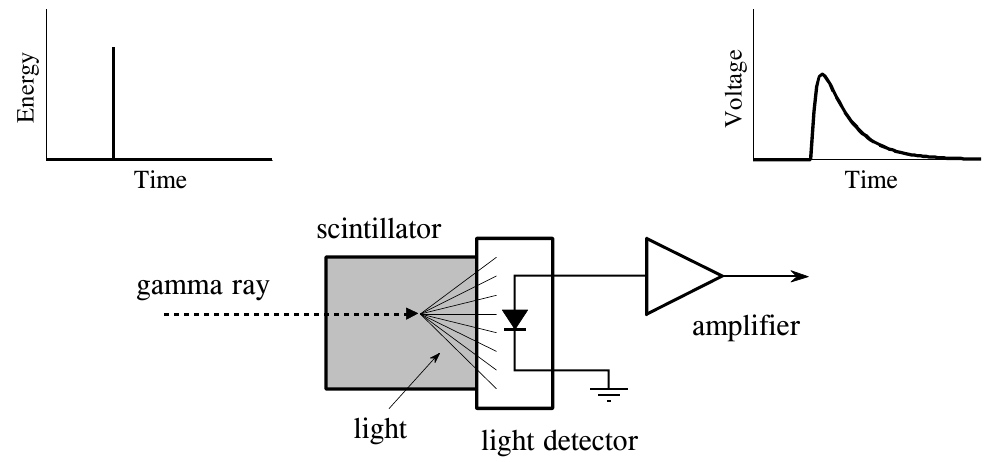
\includegraphics[width=0.833\linewidth,height=0.8\textheight,keepaspectratio]{assets/ch17/fig17-03.png}
\caption*{\textbf{图 17-3　无法避免的卷积的例子。}
把闪烁体装在光探测器上，就构成一个伽马射线探测器。伽马射线击中闪烁体时，它的能量被转换成一个光脉冲。这个光脉冲再由光探测器转换成电信号。伽马射线是一个冲激，而探测器的输出（即冲激响应）像一个单边指数函数。
（Energy = 能量，Voltage = 电压，Time = 时间；gamma ray =
伽马射线，scintillator = 闪烁体，light = 光，light detector =
光探测器，amplifier = 放大器。）}
\end{figure}

图 17-4a
是探测器对随机到达的伽马射线产生的脉冲。我们想从这个输出信号中提取的信息是每个脉冲的幅度，它与产生该脉冲的伽马射线的能量成正比。这个信息很有用，因为能量可以告诉我们这个伽马射线来自何处的有趣信息。例如，它可以提供病人的医学信息，告诉我们一个遥远星系的年龄，在航空行李中发现炸弹，等等。

如果只是偶尔探测到一个伽马射线，一切都好办，但实际情况通常不是这样。如
(a)
所示，两个或更多脉冲可能重叠，使测得的幅度发生偏移。解决这个问题的一个办法是对探测器的输出信号做反卷积，让脉冲变窄，从而减少堆积(pile-up)。理想情况下，我们希望每个脉冲都像原来的冲激。你大概也猜到了，这做不到，我们只能退而求其次，接受一个长度有限、但比探测到的脉冲短得多的脉冲。这个目标如图
17-4b 所示。

\begin{figure}[htbp]
\centering
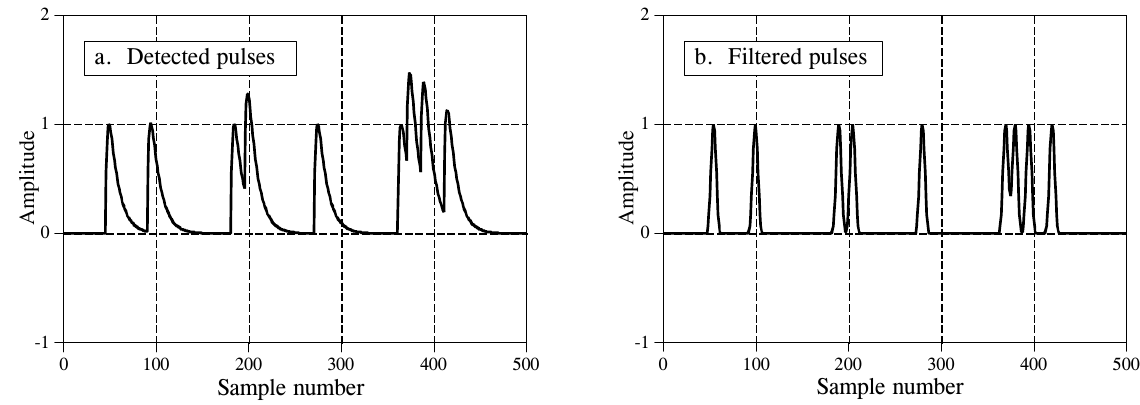
\includegraphics[width=0.950\linewidth,height=0.8\textheight,keepaspectratio]{assets/ch17/fig17-04.png}
\caption*{\textbf{图 17-4　反卷积的例子。} (a)
是伽马射线探测器对一串随机到达的伽马射线的输出信号。反卷积滤波器的设计目标是把
(a) 变成
(b)，即缩小脉冲的宽度。这样当脉冲相互叠在一起时，幅度的偏移就最小。 （a.
Detected pulses = 探测到的脉冲；b. Filtered pulses =
滤波后的脉冲。Amplitude = 幅度，Sample number = 采样序号。）}
\end{figure}

尽管探测器信号的信息编码在时域里，我们的大部分分析却必须在频域里进行，因为在那里问题更容易理解。图
17-5a 是探测器产生的信号（这是我们已知的）。(c)
是我们希望得到的信号（也是已知的）。这个期望的脉冲是随意选的，形状与布莱克曼窗相同，长度约为原脉冲的三分之一。我们的目标是找到一个滤波器核
(e)，使它与 (a) 中的信号卷积后产生 (c) 中的信号。写成公式：若
\(a * e = c\)，已知 a 和 c，求 e。

如果这些信号是用加法或乘法而不是卷积组合起来的，解法就很容易：用减法来''去加''，用除法来''去乘''。卷积则不同，并没有一种可以叫做''去卷积''的简单逆运算。卷积太复杂，无法通过直接操纵时域信号来撤销。

幸运的是，这个问题在频域里更简单。记住，一个域中的卷积对应另一个域中的乘法。仍以图
17-5 中的信号为例：若 \(b \times f = d\)，已知 b 和 d，求
f。这个问题很容易解：滤波器的频率响应 (f)，等于期望脉冲的频谱 (d)
除以探测到的脉冲的频谱
(b)。由于探测到的脉冲不对称，它的相位不为零。这意味着必须用复数除法（即一个幅度和相位除以另一个幅度和相位）。万一你忘了，第
9 章讲过怎样用一个频谱去除另一个频谱。然后用自定义滤波器的方法（逆
DFT、平移、截断、乘以窗函数），由这个频率响应求出所需的滤波器核 (e)。

\begin{figure}[htbp]
\centering
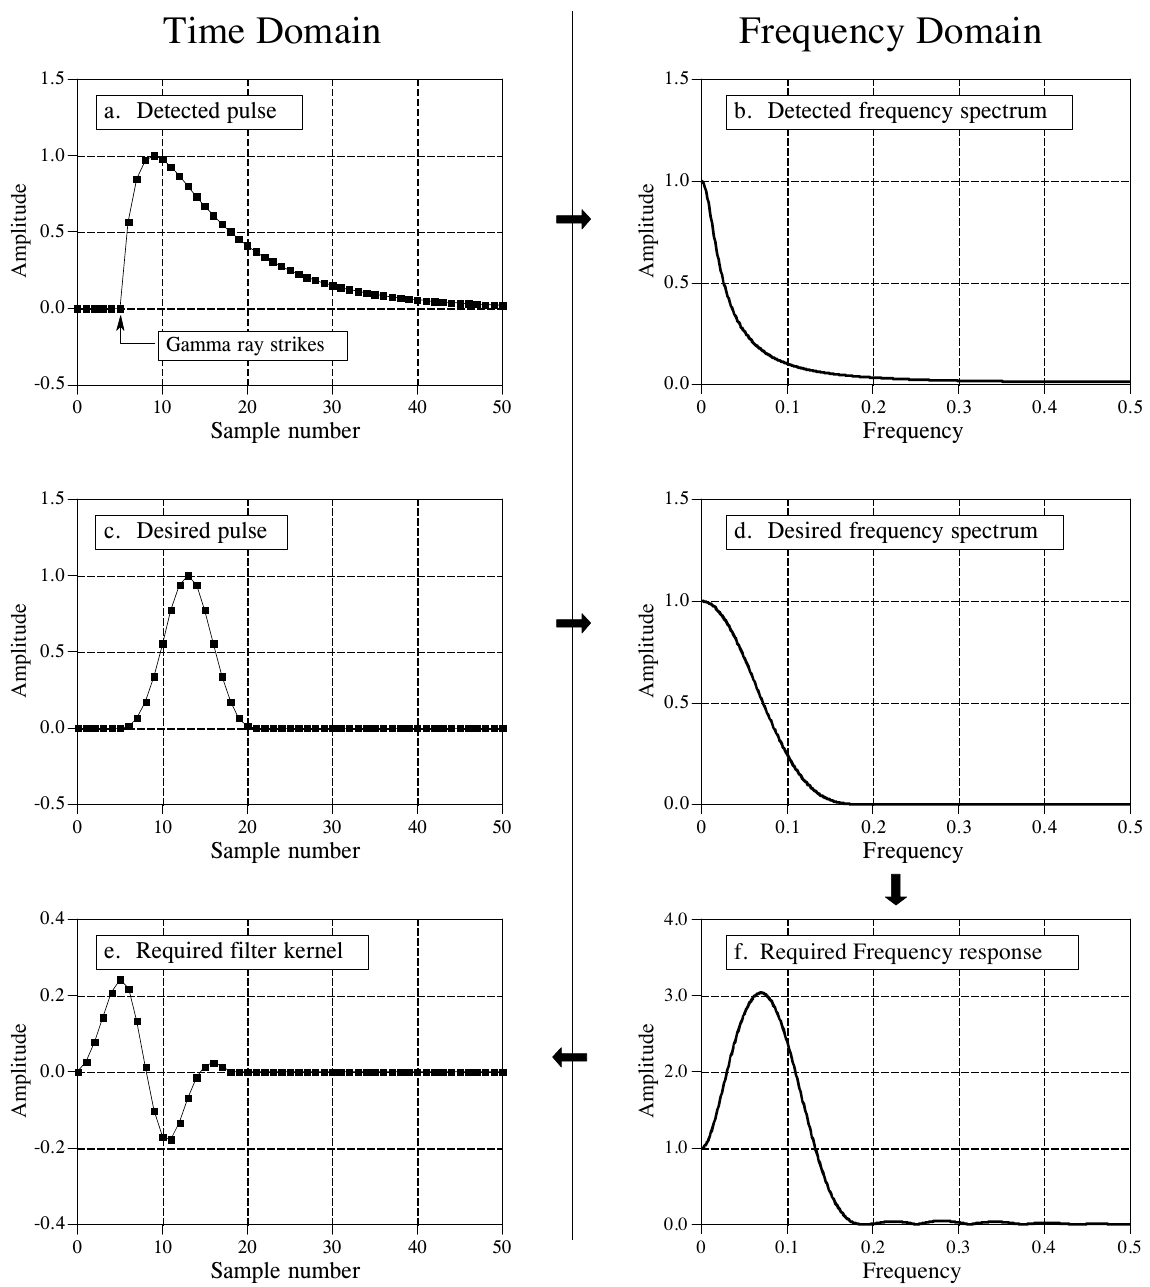
\includegraphics[width=0.958\linewidth,height=0.8\textheight,keepaspectratio]{assets/ch17/fig17-05.png}
\caption*{\textbf{图 17-5　时域和频域中的反卷积示例。}
示例伽马射线探测器的冲激响应如 (a) 所示，期望的冲激响应如 (c)
所示。这两个信号的频谱分别如 (b) 和 (d) 所示。把 (a) 变成 (c)
的滤波器，其频率响应 (f) 等于 (d) 除以 (b)。这个滤波器的核 (e)
再用自定义滤波器设计方法（逆
DFT、截断、加窗）由频率响应求出。本图只画出了频域信号的幅度；不过，它们的相位并不为零，也必须用上。
（Time Domain = 时域，Frequency Domain = 频域；a. Detected pulse =
探测到的脉冲，Gamma ray strikes = 伽马射线击中；b. Detected frequency
spectrum = 探测到的频谱；c.~Desired pulse = 期望的脉冲；d.~Desired
frequency spectrum = 期望的频谱；e. Required filter kernel =
所需的滤波器核；f.~Required Frequency response =
所需的频率响应。Amplitude = 幅度，Sample number = 采样序号，Frequency =
频率。）}
\end{figure}

\begin{quote}
\textbf{译注：} 原书图注写的是 ``(f), equal to (b) divided by (d)''，即
(b) 除以 (d)，与正文矛盾，也与图对不上：(f) 在低频处约为 1、在 0.07
附近升到约 3，只有 (d)/(b) 才是这样。这里按正文改为 (d) 除以 (b)。
\end{quote}

反卷积能带来的改善是有限度的。换句话说，如果你贪心，事情就会崩溃。在这个例子里，贪心就是想让期望的脉冲窄得过分。我们来看看会发生什么。如果期望脉冲做得更窄，它的频谱就必须包含更多的高频成分。由于这些高频成分在探测到的脉冲中幅度非常低，滤波器在这些频率上就必须有非常高的增益。例如，(f)
显示，为了得到 (c) 中的期望脉冲，有些频率必须乘以
3。如果期望脉冲做得更窄，反卷积滤波器在高频处的增益还要更大。

问题在于，在这种情况下，小误差是非常不可原谅的。例如，如果某个频率只需要放大
28 倍，却被放大了 30
倍，反卷积后的信号很可能一团糟。当反卷积被推向更高的性能水平时，对那个不想要的卷积的特性就必须了解得更准确、更精确。在现实应用中，总存在一些未知因素，来源于这样一些坏蛋：电子噪声、温度漂移、器件之间的差异等。这些未知因素限制了反卷积能做到多好。

即使完全了解那个不想要的卷积，仍然有一个因素限制反卷积的性能：噪声。例如，大多数不想要的卷积都表现为低通滤波器，降低信号中高频成分的幅度。反卷积通过放大这些频率来纠正这一点。然而，如果这些成分的幅度降到了系统固有噪声之下，这些频率中包含的信息就丢失了。再多的信号处理也找不回来。它永远消失了。Adios！Goodbye！Sayonara！试图找回这些数据只会放大噪声。极端情况下，有些频率的幅度可能完全降为零。这不仅抹掉了信息，还会使反卷积滤波器在这些频率上试图有无穷大的增益。解决办法是：设计一个不那么激进的反卷积滤波器，和/或限制任何频率上所允许的增益。

能走多远？多贪才算太贪？这完全取决于你要解决的问题。如果信号表现良好、噪声低，大概可以获得显著的改善（想想
5～10
倍）。如果信号随时间变化、了解得不是特别清楚、或者噪声大，效果就会差得多（想想
1～2
倍）。成功的反卷积需要大量的测试。如果在某个程度上奏效了，就再往前推一点；它崩溃的时候你自然会知道。再多的理论工作也不能让你绕过这个反复试验的过程。

反卷积也可以用于信息编码在频域中的信号。一个经典的例子是修复著名歌剧演唱家恩里科·卡鲁索（Enrico
Caruso，1873-1921）的老唱片。按现代标准，这些唱片是用非常原始的设备录制的。最主要的问题是用来收集声音的长管状录音喇叭的共振。每当歌手恰好唱到其中某个共振频率，录音的响度就会突然增大。数字反卷积通过压低音乐中这些过响的地方，改善了这些录音的主观听感。我们只介绍一般的方法；详细的描述请参阅原始论文：T.
Stockham, T. Cannon, and R. Ingebretsen, ``Blind Deconvolution Through
Digital Signal Processing'', Proc. IEEE, vol.~63, Apr.~1975,
pp.~678-692。

\begin{figure}[htbp]
\centering
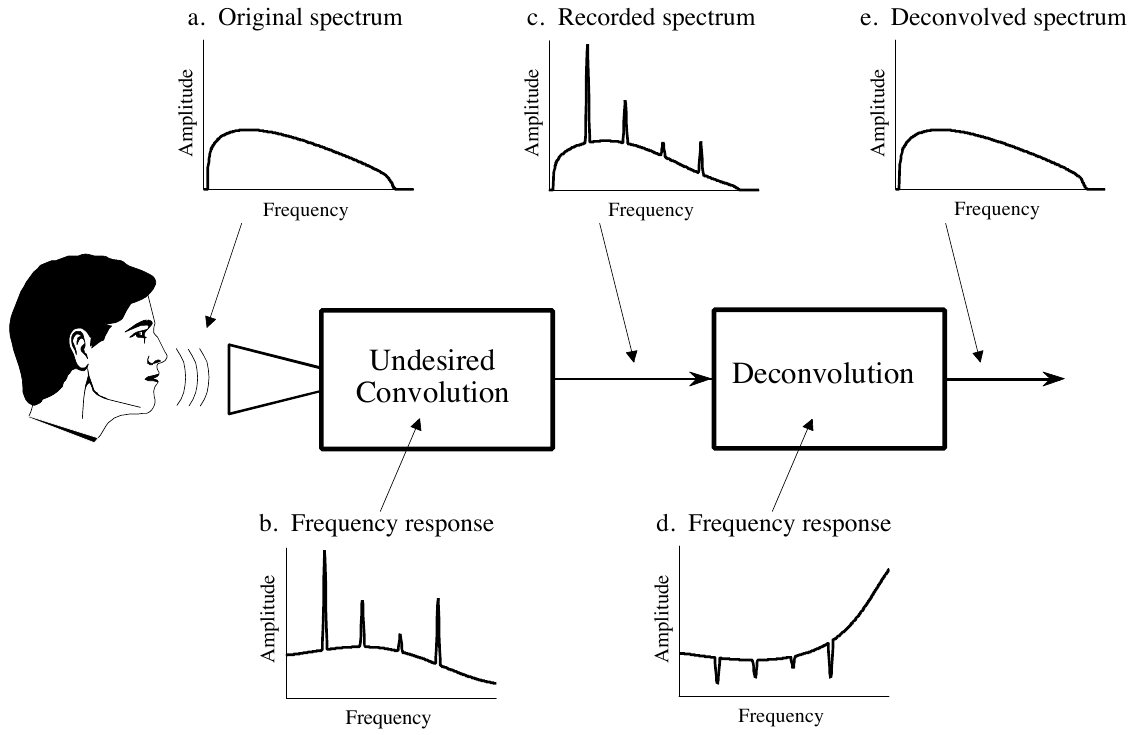
\includegraphics[width=0.950\linewidth,height=0.8\textheight,keepaspectratio]{assets/ch17/fig17-06.png}
\caption*{\textbf{图 17-6　老唱片的反卷积。} 原歌手发出的频谱如 (a)
所示。原始设备中的共振峰 (b) 使录下来的频谱 (c)
产生失真。反卷积滤波器的频率响应 (d)
用来抵消这个不想要的卷积，恢复出原始频谱
(e)。这些图仅作示意，并非真实信号。 （a. Original spectrum =
原始频谱；b. Frequency response = 频率响应；c.~Recorded spectrum =
录下的频谱；d.~Frequency response = 频率响应；e. Deconvolved spectrum =
反卷积后的频谱；Undesired Convolution = 不想要的卷积，Deconvolution =
反卷积。Amplitude = 幅度，Frequency = 频率。原书图注 ``designed to
counteracts'' 中的 counteracts 应为 counteract。）}
\end{figure}

图 17-6 展示了一般的做法。原始音频信号的频谱如 (a) 所示。(b)
是录音设备的频率响应，是一条相当平滑的曲线，只是有几个尖锐的共振峰。录下来的信号的频谱如
(c) 所示，等于真实频谱 (a) 乘以这个不平坦的频率响应
(b)。反卷积的目标是抵消这个不想要的卷积。换句话说，反卷积滤波器的频率响应
(d) 必须是 (b) 的倒数。也就是说，(b) 中的每个峰都要被 (d)
中相应的谷抵消。如果这个滤波器设计得完美无缺，得到的信号的频谱 (e)
就会与原始频谱完全相同。问题在于：原来的录音设备早就被扔掉了，它的频率响应
(b) 是个谜。换句话说，这是一个盲反卷积问题：只给出 (c)，怎样确定 (d)？

盲反卷积问题通常的解决思路，是对未知参数做出估计或假设。在这个例子中，假设原来音乐的平均频谱，与一位当代歌手用现代设备演唱同一段音乐的平均频谱相同。平均频谱用第
9 章的技术求得：把信号分成大量片段，对每个片段做
DFT，转换成极坐标形式，再把幅度平均起来。最简单的情况下，就把未知的频率响应取为老录音的平均频谱除以现代录音的平均频谱。（Stockham
等人用的方法基于一种更精巧的技术，叫同态处理(homomorphic
processing)，能更好地估计录音系统的特性。）

\section{最优滤波器}

图 17-7a
展示了一个常见的滤波问题：试图提取埋在随机噪声中的一个波形（本例中是一个指数脉冲）。如
(b)
所示，这个问题在频域中并不更容易。信号的频谱主要由低频成分组成。相比之下，噪声的频谱是白的（在所有频率上幅度相同）。由于信号和噪声的频谱相互重叠，怎样才能最好地把两者分开并不清楚。事实上，真正的问题是怎样定义''最好''。我们将看三种滤波器，每一种都在不同的意义上是''最好的''（最优的）。图
17-8 给出了这几种滤波器各自的滤波器核和频率响应。图 17-9
给出了用这些滤波器处理图 17-7a 中示例波形的结果。

\begin{figure}[htbp]
\centering
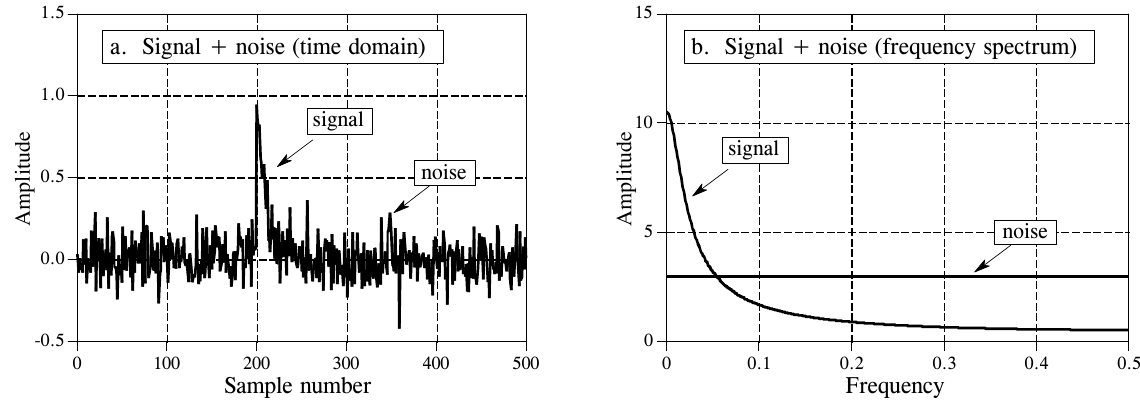
\includegraphics[width=0.950\linewidth,height=0.8\textheight,keepaspectratio]{assets/ch17/fig17-07.png}
\caption*{\textbf{图 17-7　最优滤波的例子。} (a)
是一个埋在随机噪声中的指数脉冲。脉冲和噪声的频谱如 (b)
所示。由于信号和噪声在时域和频域中都相互重叠，分离它们的最好办法并不显而易见。
（a. Signal + noise (time domain) = 信号 + 噪声（时域）；b. Signal +
noise (frequency spectrum) = 信号 + 噪声（频谱）；signal = 信号，noise =
噪声。Amplitude = 幅度，Sample number = 采样序号，Frequency = 频率。）}
\end{figure}

移动平均滤波器(moving average filter)是第 15
章的主题。你应该还记得，移动平均滤波器产生的每个输出点，都是输入信号中一定数量的点的平均值。这使得它的滤波器核是一个矩形脉冲，幅度等于参与平均的点数的倒数。移动平均滤波器的最优性在于：对于给定的降噪程度，它提供最快的阶跃响应。

匹配滤波器(matched filter)在第 7 章讨论过。如图 17-8a
所示，匹配滤波器的滤波器核与要检测的目标信号相同，只是做了左右翻转。匹配滤波器背后的思想是相关，而用卷积来实现相关需要这个翻转。输出信号中每个点的幅度，衡量的是滤波器核与输入信号相应片段的匹配程度。回想一下，匹配滤波器的输出不一定像被检测的信号。这其实无关紧要；如果用匹配滤波器，目标信号的形状肯定已经知道了。匹配滤波器的最优性在于：峰顶高出噪声的程度，比任何其他线性滤波器所能达到的都高（见图
17-9b）。

\begin{figure}[htbp]
\centering
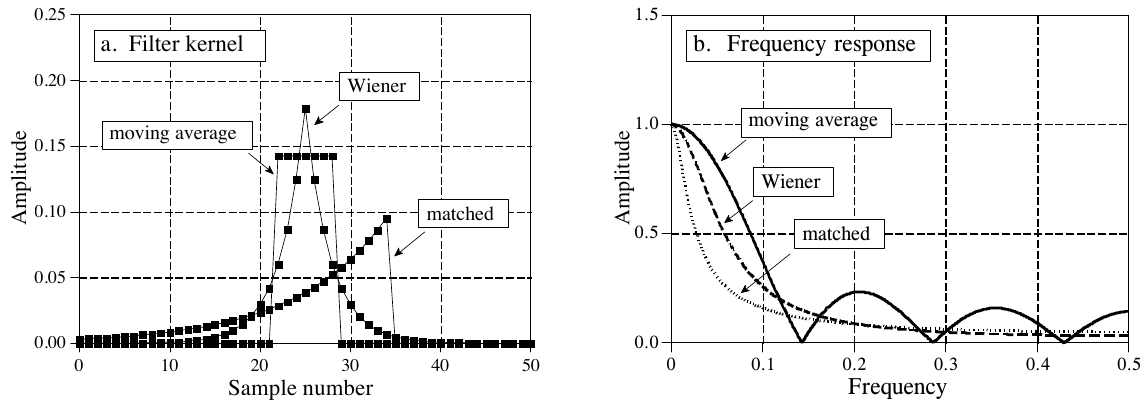
\includegraphics[width=0.954\linewidth,height=0.8\textheight,keepaspectratio]{assets/ch17/fig17-08.png}
\caption*{\textbf{图 17-8　最优滤波器的例子。} (a)
中画出了三个滤波器核，每一个都在某种意义上是最优的。相应的频率响应如 (b)
所示。移动平均滤波器被设计成以矩形脉冲为滤波器核。相比之下，匹配滤波器的核看起来像被检测的信号。维纳滤波器是在频域中设计的，依据的是每个频率上信号和噪声的相对多少。
（a. Filter kernel = 滤波器核；b. Frequency response = 频率响应；moving
average = 移动平均，Wiener = 维纳，matched = 匹配。Amplitude =
幅度，Sample number = 采样序号，Frequency = 频率。）}
\end{figure}

维纳滤波器(Wiener
filter，以诺伯特·维纳的最优估计理论命名)依据信号的频谱来分离信号。如图
17-7b
所示，在某些频率上主要是信号，在另一些频率上主要是噪声。看起来很合理的做法是：让''主要是信号''的频率通过滤波器，挡住''主要是噪声''的频率。维纳滤波器把这个思路又往前推了一步：滤波器在每个频率上的增益，由该频率上信号和噪声的相对多少决定：

\textbf{公式 17-1}　维纳滤波器。频率响应 H{[}f{]} 由噪声的频谱 N{[}f{]}
和信号的频谱 S{[}f{]} 决定。只有幅度起作用，所有相位都为零。

\[H[f] = \frac{S[f]^2}{S[f]^2 + N[f]^2}\]

用这个关系式，可以把图 17-7b 中的频谱转换成图 17-8b
中维纳滤波器的频率响应。维纳滤波器的最优性在于：它使信号功率与噪声功率之比最大（在整个信号长度上，而不是在每个单独的点上）。合适的滤波器核用自定义方法由维纳频率响应设计出来。

\begin{figure}[htbp]
\centering
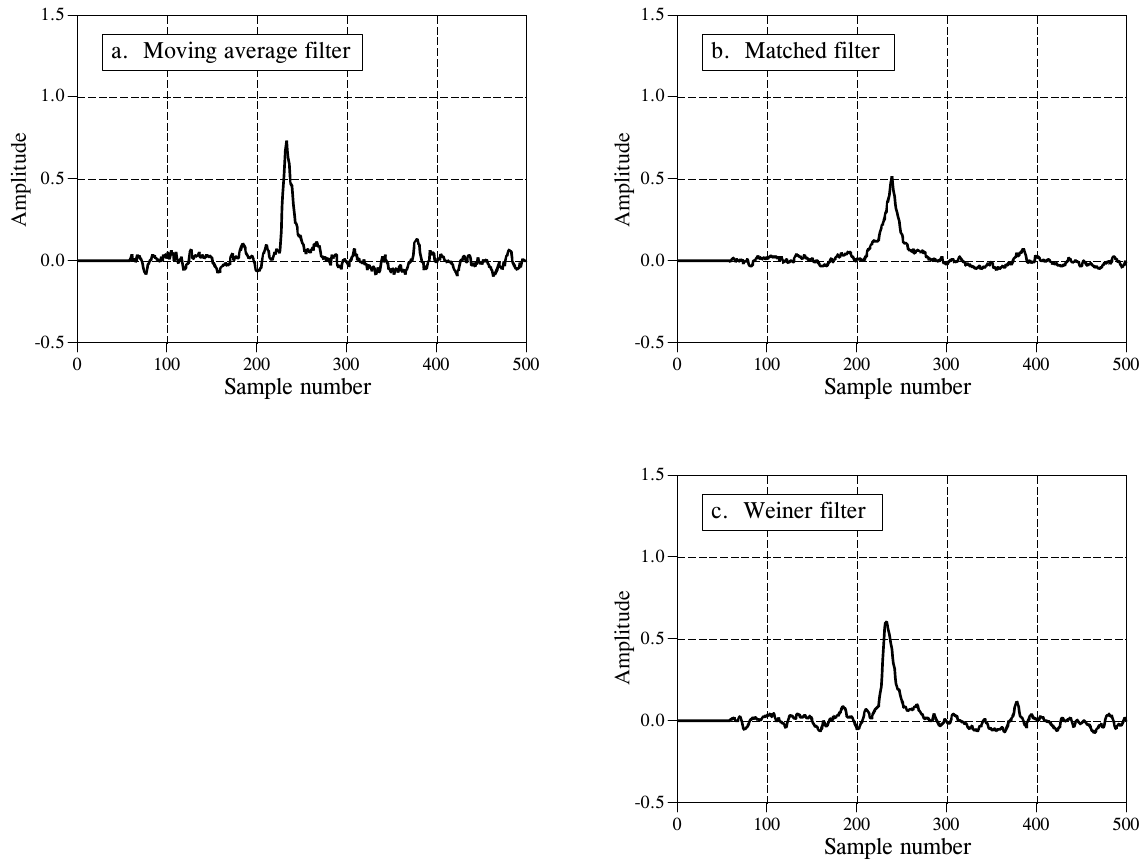
\includegraphics[width=0.950\linewidth,height=0.8\textheight,keepaspectratio]{assets/ch17/fig17-09.png}
\caption*{\textbf{图 17-9　使用三种最优滤波器的例子。} 这些信号是用图 17-8
中的滤波器对图 17-7
中的波形做滤波得到的。这三种滤波器都在某种意义上是最优的。(a)
中，对于给定的随机噪声降低程度，移动平均滤波器得到最陡峭的边缘响应。(b)
中，匹配滤波器产生的峰高出残余噪声的程度超过任何其他滤波器。(c)
中，维纳滤波器使信噪比最优。 （a. Moving average filter =
移动平均滤波器；b. Matched filter = 匹配滤波器；c.~Weiner filter =
维纳滤波器（原书把 Wiener 误拼成 Weiner）。Amplitude = 幅度，Sample
number = 采样序号。原书图注排在左下空白处，裁图时已去掉，译文见上。）}
\end{figure}

这些最优滤波器背后的思想在数学上很优雅，但在实践中常常不灵。这并不是说永远不该用它们。要点在于：别一听到''最优''二字就停止思考。我们来看几个你可能不想用它们的理由。

第一，图 17-9
中这几个信号之间的差别很不起眼。事实上，如果没人告诉你优化的是哪个参数，光看这些信号你大概分辨不出来。对于频谱重叠的问题，通常都是这样。最优滤波器带来的那一点额外性能，可能抵不上增加的程序复杂度、额外的设计工作量或更长的执行时间。

第二，维纳滤波器和匹配滤波器完全由问题本身的特性决定。其他滤波器，比如加窗
sinc
滤波器和移动平均滤波器，可以按你的喜好调整。最优滤波器的拥护者会说，这种摆弄只会降低滤波器的效果。这一点很值得商榷。记住，这些滤波器中的每一种都只在某一个特定的方面是最优的（即''在某种意义上''）。这很少足以说明整个问题都被优化了，尤其是当得到的信号要由人来解读的时候。例如，一位生物医学工程师可能用维纳滤波器来使心电图的信噪比最大。然而，这是否同时使医生通过看信号来发现心律异常的能力也达到最优，并不明显。

第三，维纳滤波器和匹配滤波器必须用卷积来实现，执行起来极慢。即使用下一章讨论的提速方法（FFT
卷积），计算时间也可能长得过分。相比之下，递归滤波器（比如移动平均滤波器或第
19 章介绍的其他滤波器）要快得多，而且可能提供可以接受的性能。
